\section{results}
    \subsection{Internal Evaluation on Expert Dataset}

        The trained Random Forest classifier was internally evaluated using an expert-labeled dataset. The dataset was partitioned into training and validation subsets using an 80:20 split. Table~\ref{tab:classification_report} presents the classification performance metrics obtained on the validation set.

        \begin{table}[h]
        \centering
        \caption{Classification Report on Validation Data}
        \label{tab:classification_report}
        \begin{tabular}{|c|c|c|c|c|}
        \hline
        \textbf{Class} & \textbf{Precision} & \textbf{Recall} & \textbf{F1-Score} & \textbf{Support} \\
        \hline
        \texttt{bb} & 0.85 & 0.85 & 0.85 & 48 \\
        \texttt{gg} & 0.95 & 0.95 & 0.95 & 137 \\
        \hline
        \textbf{Accuracy} & \multicolumn{4}{c|}{0.92 (185 samples)} \\
        \textbf{Macro Avg} & 0.90 & 0.90 & 0.90 & 185 \\
        \textbf{Weighted Avg} & 0.92 & 0.92 & 0.92 & 185 \\
        \hline
        \end{tabular}
        \end{table}

        The results indicate an overall accuracy of \textbf{92\%}, with the \texttt{gg} class achieving slightly higher precision and recall compared to the \texttt{bb} class.

        To identify the most influential sensor parameters contributing to the classification decisions, feature importance scores were extracted from the trained Random Forest model. Table~\ref{tab:feature_importance} lists the top two most significant features.

        \begin{table}[h]
        \centering
        \caption{Top Influential Features Based on Importance Scores}
        \label{tab:feature_importance}
        \begin{tabular}{|c|c|}
        \hline
        \textbf{Feature} & \textbf{Importance Score} \\
        \hline
        \texttt{RUN\_TIME} & 0.7149 \\
        \texttt{Timestamp\_OBD} & 0.2851 \\
        \hline
        \end{tabular}
        \end{table}

        A visual representation of feature importance is depicted in Fig.~\ref{fig:feature_importance}. The plot highlights that \texttt{RUN\_TIME} is the most dominant feature influencing the classification output.

        \begin{figure}[h]
        \centering
        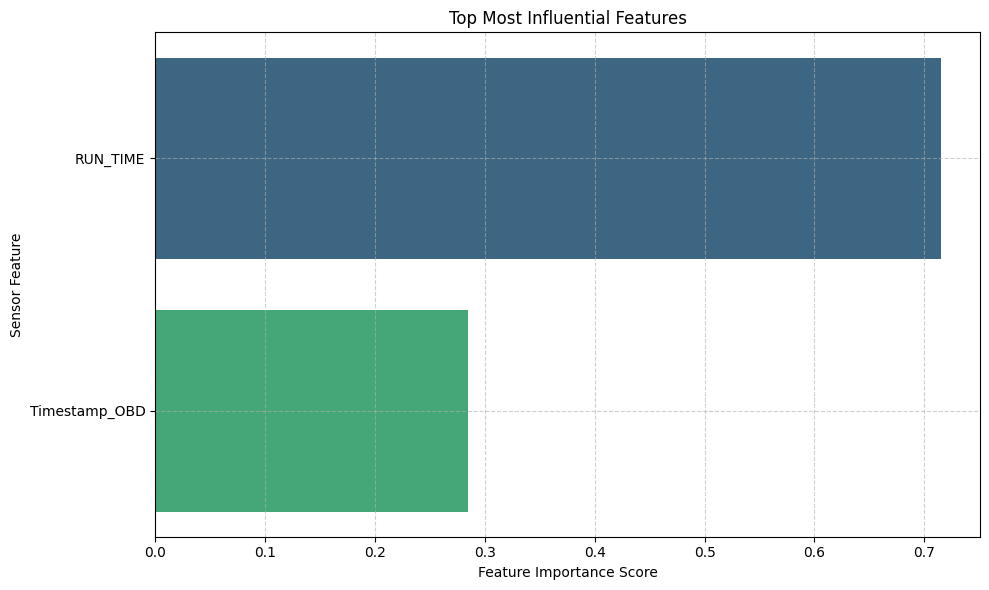
\includegraphics[width=0.45\textwidth]{assets/feature_importance.png} % replace with actual image file
        \caption{Top Sensor Features Influencing Model Predictions}
        \label{fig:feature_importance}
        \end{figure}

        During visualization, a future deprecation warning from the Seaborn library was noted regarding the use of the \texttt{palette} parameter without an accompanying \texttt{hue} assignment. This issue will be addressed in subsequent revisions to maintain compatibility with future library updates.

        \textbf{Summary:} The classifier demonstrated high predictive performance on expert data, with \texttt{RUN\_TIME} emerging as the most critical sensor parameter influencing engine condition classification.

    \subsection{Prediction Results and Distribution Analysis}
        After deploying the trained engine condition classification model on real-world sensor data obtained from the \texttt{Breeza\_bits.csv} dataset, the following results were observed.

        The model expects two input features for prediction:
        \begin{itemize}
            \item \texttt{Timestamp\_OBD}
            \item \texttt{RUN\_TIME}
        \end{itemize}

        The test dataset was cleaned to remove missing values and the required features were extracted accordingly. Predictions were then performed using the loaded model.

        The distribution of predicted class labels is presented in Table~\ref{tab:prediction_count}. It indicates the frequency of each predicted condition label within the test dataset.

        \begin{table}[h]
        \centering
        \caption{Prediction Count Per Class}
        \label{tab:prediction_count}
        \begin{tabular}{|c|c|}
        \hline
        \textbf{Label} & \textbf{Count} \\
        \hline
        gg (Good) & 675 \\
        bb (Bad)  & 249 \\
        \hline
        \end{tabular}
        \end{table}

        A visual representation of the prediction distribution is shown in Fig.~\ref{fig:prediction_distribution}. This bar chart highlights the number of occurrences for each predicted class label.

        \begin{figure}[h]
        \centering
        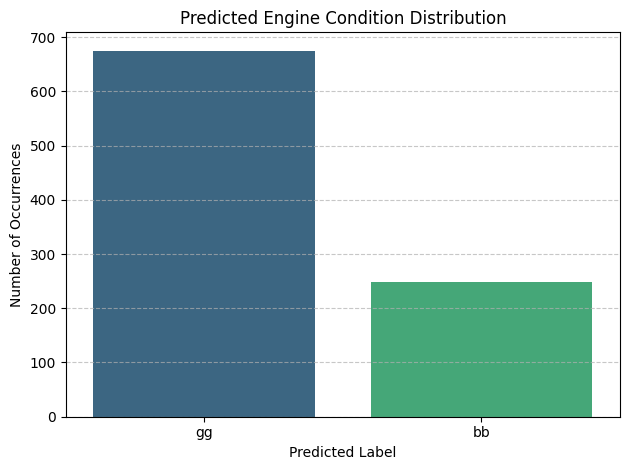
\includegraphics[width=0.45\textwidth]{assets/prediction_distribution.png} % replace with actual image file
        \caption{Predicted Engine Condition Distribution}
        \label{fig:prediction_distribution}
        \end{figure}

        During visualization, a future deprecation warning was noted in the Seaborn library indicating that passing the \texttt{palette} parameter without a corresponding \texttt{hue} assignment will be deprecated in version 0.14.0. This will be addressed in future implementation updates to ensure compatibility.

        Based on the prediction results:
        \begin{itemize}
            \item The majority of instances (675) were classified as \texttt{gg} (Good condition)
            \item 249 instances were classified as \texttt{bb} (Bad condition)
        \end{itemize}
        Hence, it can be concluded that the overall condition status of the test dataset is \textbf{Good}, as the number of healthy predictions outweighs the fault detections.
